\documentclass[11pt]{amsart}

\usepackage[english]{babel}
\usepackage{appendix}
\usepackage{amsmath}
\usepackage{amsfonts}
\usepackage{amssymb}
%\usepackage{showlabels}
\usepackage{hyperref}
\usepackage{amsthm}
\usepackage{marginnote}
\usepackage{stmaryrd}
\usepackage{enumitem}
\usepackage[english]{babel}
\usepackage{yfonts}
\usepackage[T1]{fontenc}
\usepackage[utf8x]{inputenc}

\usepackage{calrsfs}
\DeclareMathAlphabet{\pazocal}{OMS}{zplm}{m}{n}

\usepackage{verbatim}
\usepackage{graphicx}
\usepackage{verbatim}
\usepackage{faktor}
\usepackage{xcolor}
\usepackage{xfrac}
\usepackage{tikz,tikz-cd}
\usetikzlibrary{decorations.pathmorphing,decorations.pathreplacing,patterns}

\usepackage[all]{xy}
\usepackage{bbm}
\usepackage{tabularx}
\usepackage{longtable}
\usepackage{tabu}
\usepackage{booktabs}
\usepackage{mathtools}

\usepackage[]{textcomp}
\usepackage[sups]{Baskervaldx}
\usepackage{cabin}
\usepackage[varqu,varl]{inconsolata}
\usepackage[baskervaldx,bigdelims,vvarbb]{newtxmath}
\usepackage[cal=cm]{mathalfa}


\newcommand{\plC}{\scalebox{0.8}[1.3]{$\sqsubset$}}
\newcommand{\sidenote}[1]{\marginpar{\textbf{\color{red}#1}}}

\def\Yagraph{\tikz[baseline=-3pt,scale=.8]{
\draw (2,0) -- (0,1) (2,0) -- (0,.5) (2,0) -- (0,-1);
\draw (2,0) circle(2pt)[fill=black];
\draw (0,1) circle(2pt)[fill=white];
\draw (0,.5) circle(2pt)[fill=black];
\draw (0,-.5) node{$\ldots$};
\draw (0,-1) circle(2pt)[fill=black];
\draw (-1,1.5) -- (1,1.5) -- (1,-1.5) -- (-1,-1.5) -- (-1,1.5);
\draw (1,1.5) -- (3,2) -- (3,-1) -- (1,-1.5);
}}

\def\Ybgraph{\tikz[baseline=-3pt,scale=.8]{
\draw (2,0) to[out=120,in=0] (0,1) (2,0) -- (0,1) (2,0) -- (0,.5) (2,0) -- (0,-1);
\draw (2,0) circle(2pt)[fill=black];
\draw (0,1) circle(2pt)[fill=black];
\draw (0,.5) circle(2pt)[fill=black];
\draw (0,-.5) node{$\ldots$};
\draw (0,-1) circle(2pt)[fill=black];
\draw (-1,1.5) -- (1,1.5) -- (1,-1.5) -- (-1,-1.5) -- (-1,1.5);
\draw (1,1.5) -- (3,2) -- (3,-1) -- (1,-1.5);
}}

\def\Ycgraph{\tikz[baseline=-3pt,scale=.8]{
\draw (2,0) -- (0,1) (2,0) -- (0,.5) (2,0) -- (0,-1);
\draw (2,0) circle(2pt)[fill=white];
\draw (0,1) circle(2pt)[fill=black];
\draw (0,.5) circle(2pt)[fill=black];
\draw (0,-.5) node{$\ldots$};
\draw (0,-1) circle(2pt)[fill=black];
\draw (-1,1.5) -- (1,1.5) -- (1,-1.5) -- (-1,-1.5) -- (-1,1.5);
\draw (1,1.5) -- (3,2) -- (3,-1) -- (1,-1.5);
}}

\newcommand{\mathsq}[1]{#1}
\newcommand{\pM}{\pazocal{M}}
\newcommand{\TT}{\operatorname{T}}
\newcommand{\oM}{\overline{\mathcal{M}}}
\newcommand{\M}[4]{\overline{\mathcal{M}}_{#1,#2}(#3,#4)}
\newcommand{\MG}[4]{\overline{\mathcal{M}}^{\rm G}_{#1,#2}(#3,#4)}
\newcommand{\Q}[4]{\mathcal{Q}_{#1,#2}(#3,#4)}
\newcommand{\Qe}[4]{\mathcal{Q}^{\epsilon}_{#1,#2}(#3,#4)}
\newcommand{\Qt}[4]{\widetilde{\mathcal Q}_{#1,#2}(#3,#4)}
\newcommand{\QG}[4]{\mathcal{Q}G_{#1,#2}(#3,#4)}
\newcommand{\QGe}[4]{\mathcal{Q}G^{\epsilon}_{#1,#2}(#3,#4)}
\newcommand{\D}[3]{\mathcal{D^Q}(#1,#2,#3)}
\newcommand{\E}[3]{\mathcal{E^Q}(#1,#2,#3)}
\newcommand{\PP}{\mathbb P}
\newcommand{\Z}{\mathbb{Z}}
\newcommand{\VZ}{\pazocal{V\!Z}}
\newcommand{\tVZc}[4]{\widetilde{\mathcal{V\!Z}}^{\rm{ctr}}_{#1,#2}(#3,#4)}
\newcommand{\VZc}[4]{\mathcal{V\!Z}_{#1,#2}(#3,#4)}
\newcommand{\VZcLi}[4]{\mathcal{V\!Z}^{\rm{ctr, Li}}_{#1,#2}(#3,#4)}
\newcommand{\VZrel}[4]{\mathcal{V\!Z}^{\rm{rel}}_{#1,#2}(#3,#4)}
\newcommand{\stab}{\rm{stab}}
\newcommand{\stC}{C'}
\newcommand{\stf}{f'}
\newcommand{\stpi}{\pi'}
\newcommand{\sts}{s'}
\newcommand{\N}{\mathbb{N}}
\newcommand{\OO}{\mathcal{O}}
\renewcommand{\to}{\rightarrow}
\newcommand{\A}{\mathcal A}
\newcommand{\B}{\mathcal B}
\newcommand{\C}{\mathfrak C}
\newcommand{\cC}{\mathcal C}
\newcommand{\EE}{\mathbf{E}}
\renewcommand{\L}{\mathcal L}
\newcommand{\LL}{\mathbf{L}}
\newcommand{\MM}{\mathfrak M}
\newcommand{\Aaff}{\mathbb{A}}
\newcommand{\kfield}{\Bbbk}
\newcommand{\comp}{\chi}
\newcommand{\sst}{\sigma^{\operatorname{ss}}}
\newcommand{\Pic}{\operatorname{Pic}}
\newcommand{\Def}{\operatorname{Def}}
\newcommand{\Spec}{\operatorname{Spec}}
\newcommand{\Proj}{\operatorname{Proj}}
\newcommand{\Hom}{\operatorname{Hom}}
\newcommand{\Ext}{\operatorname{Ext}}
\newcommand{\Gm}{\mathbb{G}_{\text{m}}}
\newcommand{\virt}[1]{[#1]^{\operatorname{virt}}}
\newcommand{\vip}[1]{[#1]^{\operatorname{prod}}}
\newcommand{\Id}{\operatorname{Id}}
\newcommand{\CC}{\mathbb{C}}
\newcommand{\QQ}{\mathbb{Q}}
\newcommand{\HH}{\operatorname{H}}
\newcommand{\Achow}{\operatorname{A}}
\newcommand{\pt}{\operatorname{pt}}
\newcommand{\bq}{\begin{equation}}
\newcommand{\eq}{\end{equation}}
\newcommand{\ba}{\begin{aligned}}
\newcommand{\ea}{\end{aligned}}
\newcommand{\be}{\begin{enumerate}}
\newcommand{\ee}{\end{enumerate}}
\newcommand{\bsm}{\left(\begin{smallmatrix}}
\newcommand{\esm}{\end{smallmatrix}\right)}                   
\newcommand{\bpm}{\begin{pmatrix}}
\newcommand{\epm}{\end{pmatrix}}
\newcommand{\barr}{\begin{displaymath}\begin{array}{cccc}}
\newcommand{\earr}{\end{array}\end{displaymath}}
\newcommand{\barrl}{\begin{displaymath}\begin{array}{lcl}}
\newcommand{\earrl}{\end{array}\end{displaymath}}
\newcommand{\barl}{\begin{displaymath}\begin{array}{l}}
\newcommand{\earl}{\end{array}\end{displaymath}}
\newcommand{\bxym}{ \begin{displaymath}\xymatrix }
\newcommand{\exym}{\end{displaymath}}
\newcommand{\bcd}{\begin{center}\begin{tikzcd}}
\newcommand{\ecd}{\end{tikzcd}\end{center}}
\newcommand{\R}{\operatorname{R}^{\bullet}}
\newcommand{\dvr}{\Delta}
%\newcommand{\sslash}{\mathbin{/\mkern-6mu/}}
\newcommand{\tr}{{\rm tr}}
\newcommand{\Isom}{\text{Isom}}
\newcommand{\pr}{\operatorname{pr}}
\newcommand{\ev}{\operatorname{ev}}
\newcommand{\fgt}{\operatorname{fgt}}
\newcommand{\codim}{\operatorname{codim}}
\newcommand{\vdim}{\operatorname{vdim}}
\newcommand{\ildef}[1]{\emph{#1}}
\newcommand{\om}[1]{\mathcal{#1}}
\newcommand{\h}{\operatorname{h}}
\newcommand{\Aut}{\operatorname{Aut}}
\newcommand{\Acal}{\mathcal{A}}
\newcommand{\Mcal}{\mathcal{M}}
\newcommand{\ol}[1]{\overline{#1}}
\newcommand{\op}[1]{\operatorname{#1}}
\newcommand{\gp}{\operatorname{gp}}
\newcommand{\RR}{\mathbb{R}}
\newcommand{\NN}{\mathbb{N}}
\newcommand{\ovm}[1]{\overline{\mathcal{#1}}}
\newcommand{\ovt}[1]{\widetilde{\mathcal{#1}}}
\newcommand{\ov}[1]{\overline{#1}}

\theoremstyle{definition}
\newtheorem{thm}{Theorem}[section]
\newtheorem{lem}[thm]{Lemma}
\newtheorem{lemma}[thm]{Lemma}
\newtheorem{prop}[thm]{Proposition}
\newtheorem{cor}[thm]{Corollary}
\newtheorem*{teo*}{Theorem}
\newtheorem{ipotesi}{ipotesi}
\newtheorem*{nota}{Nota}
\newtheorem{claim}{Claim}
\newtheorem{question}[thm]{Question}
\newtheorem{conj}[thm]{Conjecture}

\newtheorem{innercustomthm}{Theorem}
\newenvironment{customthm}[1]
  {\renewcommand\theinnercustomthm{#1}\innercustomthm}
  {\endinnercustomthm}

\theoremstyle{definition}
\newtheorem{example}[thm]{Example}
\newtheorem{ex}[thm]{Example}
\newtheorem{dfn}[thm]{Definition}
\newtheorem{definition}[thm]{Definition}
\newtheorem{aside}[thm]{Aside}
\newtheorem{remark}[thm]{Remark}
\newtheorem{com}[thm]{Comment}
\newtheorem{num}{Number}
\newtheorem*{sketch}{Sketch}
\newtheorem*{rem}{Remark}
\newtheorem*{aside*}{Aside}
\newtheorem*{acknowledgements}{Acknowledgements}

\newcommand{\ilemph}[1]{\emph{#1}}

\setcounter{tocdepth}{1}

\newcommand{\todo}[1]{\vspace{5mm}\par \noindent
\framebox{\begin{minipage}[c]{0.95 \textwidth} \tt #1\end{minipage}} \vspace{5mm} \par}

\def\ti{-\allowhyphens}
\newcommand{\thismonth}{\ifcase\month % case 0 --- impossible!
  \or January\or February\or March\or April\or May\or June%
  \or July\or August\or September\or October\or November%
  \or December\fi}
\newcommand{\thismonthyear}{{\thismonth} {\number\year}}
\newcommand{\thisdaymonthyear}{{\number\day} {\thismonth} {\number\year}}

\title[Genus One Reduced Relative Invariants]{Relative Stable Maps in Genus One via Central Alignments}
\author{Luca Battistella, Navid Nabijou and Dhruv Ranganathan}
\date{\thismonthyear}

\begin{document}


\begin{abstract} For a smooth projective variety $X$ and a smooth very ample hypersurface $Y \subseteq X$, we define moduli spaces of relative stable maps to $(X,Y)$ in genus one, as closed substacks of the moduli space of maps from centrally aligned curves, constructed in \cite{RSPW}. We construct virtual classes for these moduli spaces, which we use to define \emph{reduced relative Gromov--Witten invariants} in genus one.

[GOALS: We prove a recursion formula which allows us to completely determine these invariants in terms of the reduced Gromov--Witten invariants, as defined in [REF]. We also prove a relative version of the Li--Zinger formula, relating our invariants to the usual relative Gromov--Witten invariants. Also say something about quasimaps.]
\end{abstract}

\maketitle

\appendixtitletocoff
\tableofcontents

\section{Introduction}

\subsection{Statement of the problem} Contrary to the genus zero case, the moduli space of genus one maps to projective space - with or without markings - is far from smooth; indeed it has various boundary components of different dimensions, representing maps that contract a genus one curve and have all the degree supported on a number of rational tails. The many incarnations of relative moduli spaces also suffer of the same undesirable feature.

Since the work of Vakil--Zinger and Ranganathan--Santos-Parker--Wise, it has been clear that it is possible to identify a desingularisation of the main component by adding the extra data of a contraction of the source curve $\nu\colon C\to \bar{C}$ - where the latter is allowed to acquire a Smyth singularity - and requiring the stable map $f\colon C\to \PP^N$ to factor through $\nu$.

\subsection{Choice of relative space and desingularisation} We focus on the space of logarithmic stable maps to $(\PP^N|H)$, following ACGS. We perform a log modification of this space as detailed below. For a log curve $C\to S=\Spec(k=\bar k)$, modify the dual graph of $C$ by replacing the minimal genus one subcurve (in case it is a circle of $\PP^1$) by a single vertex of genus one, called the \emph{core} and denoted by $\circ$, and define a piecewise linear function with values in $\overline{\pazocal M}_S$ on such a graph by setting \[\lambda(v)=\sum_{q\in[\circ,v]}\rho_q,\]
where the $\rho_q$ are the smoothing parameters of the nodes $q$ separating $v$ from the core. Such a function is related to the log canonical bundle of $C\to S$. When the map contracts a subcurve of genus one, we endow it with the extra data of a radius $\delta\in\overline{\pazocal M}_S$ subject to the following compatibility condition:

(*) \emph{the circle of radius $\delta$ around $\circ$ passes through $\geq1$ vertex of positive $f$-degree}.

\noindent Furthermore, we require all the values of $\lambda$ to be comparable with $\delta$, and among themselves whenever they are $\leq \delta$. This is called a \emph{centrally aligned} log structure and carries enough information to define a contraction $\nu\colon C\to \bar{C}$, possibly after a semistabilisation of $(C,f)$ - in fact even more. The space thus obtained, $\widetilde \VZ_{1,\alpha}(\PP^N|H,d)$, is a log modification of $\M{1}{\alpha}{\PP^N|H}{d}$.

The main component $\VZ_{1,\alpha}(\PP^N|H,d)$ is then identified by a double factorisation condition:
\begin{enumerate}
 \item If $f$ contracts a genus one subcurve, then $f$ is required to factor through the Smyth singularity $\nu\colon C\to \bar C$ determined by the contraction radius $\delta$ as above.
 \item If furthermore the core is contracted by the associated tropical map $\phi$, let $\delta_2$ be the minimal distance from $\circ$ to a vertex supporting a flag that escapes $\phi^{-1}(\phi(\circ))$; we require $f$ to factor through $\nu_2\colon C\to\bar C_2$.
\end{enumerate}
The main result is that
\begin{thm}
 $\VZ_{1,\alpha}(\PP^N|H,d)$ is (log) smooth.
\end{thm}

\subsection{Gathmann-type recursion} There is a forgetful morphism \[\VZ_{1,\alpha}(\PP^N|H,d)\to \VZ_{1,n}(\PP^N,d),\] hitting Gathmann's relative space. We may therefore pullback Gathmann's line bundle and section, cutting out the locus where the $k$-th marking is tangent to $H$ to order $\alpha_k+1$. Because $\alpha$ was maximal ($\sum\alpha=d$) by assumption, this means that the curve has to break, and $x_k$ has to lie on an internal component - one which is entirely mapped into $H$. We identify the zero locus of Gathmann's section explicitly. Here is an interesting remark: the combinatorics of such boundary loci is governed by tropical geometry, and it is otherwise very hard to districate the interaction between the relative condition and the exceptional loci of the Vakil--Zinger blow-up.
\begin{cor}
 $\VZ_{1,\alpha}(\PP^N|H,d)$ is smooth over its Artin fan, in particular codimension one logarithmic strata can be read off from the latter.
\end{cor}
The Artin fan is a tropical gadget. Its local structure is given by subdividing the ACGS minimal monoid according to the alignment. We are only interested in picking its rays. The upshot is that the combinatorics is slightly more involved than in the genus zero case: the alignment may force some teeth of the comb to break.
\begin{thm}[Gathmann-type formula, maximal tangency, $(\PP^N|H)$ case]
 \[(\alpha_k\psi_k+\ev_k^*H)[\VZ_{1,\alpha}(\PP^N|H,d)]=[D_{1,\alpha;k}(\PP^N|H,d)],\]
 the latter being a sum of broken comb loci indexed by rays of the tropical fan.
\end{thm}
Importantly, the broken comb loci admit a very explicit description in terms of tautological integrals on the underlying boundary of Gathmann's relative space.
\begin{thm}
 Up to a finite cover of the underlying boundary stratum - which is a combinatorially-determined fiber product of moduli spaces of genus zero and one, absolute and relative maps with lower numerical invariants - every component of $D_{\alpha,k}(\PP^N|H,d)$ can be described as the transverse intersection of two loci in a projective bundle, where:
 \begin{itemize}
  \item the latter parametrises the possible line bundle isomorphisms imposed by the alignment of the log structure;
  \item the first locus is a subbundle representing the residual isomorphisms after fixing the ones virtually imposed by tropical continuity;
  \item the second locus is determined by the factorisation conditions.
 \end{itemize}
\end{thm}
The upshot is that we may then push the formula down to the Gathmann's space, so as to obtain multiplicities and tautological classes.
\begin{cor}
 \[(\alpha_k\psi_k+\ev_k^*H)[\VZ^G_{1,\alpha}(\PP^N|H,d)]=[D^G_{1,\alpha;k}(\PP^N|H,d)],\]
 the latter being expressible as a weighted sum of tautological classes on Gathmann's comb loci.
\end{cor}
Once we have this formula, the following extensions are classical:
\begin{itemize}
 \item A similar formula for raising the tangency holds in the non-maximal tangency case. It can be proven by adding auxiliary markings of contact order $1$; forgetting them is then a $(d-\sum\alpha)!:1$ cover because the nice locus is dense inside Gathmann's relative spaces.
 \item The formula holds more generally for any smooth projective target $X$ relative to a generic hyperplane section $Y=X\cap H\subseteq \PP^N$. This follows via virtual pullback.
\end{itemize}
Finally the recursive structure of the boundary allows us to prove the following
\begin{thm}[In-principle quantum Lefschetz]
 The restricted reduced genus one invariants of $Y$ can be inductively deducted from the full descendant genus zero and one (reduced) Gromov-Witten theory of $X$.
\end{thm}
The proof is more delicate than its genus zero analogue because invariants with the same numerical data appear intertwined in the last steps of the recursion.

\section{Desingularisation of the moduli space of log stable maps}
The ultimate goal of the paper is to apply Gathmann's techniques to the Vakil-Zinger desingularisation $\VZ_{1,n}(\PP^N,d)$ and to obtain a quantum Lefschetz result for reduced invariants under some positivity assumption. The key step is to study the unobstructed case $(\PP^N|H)$. We approach the problem by lifting it to the ACGS space of log stable maps. This allows us to exploit the tools developed in \cite{RSPW,RSPW2}. We are in an intermediate situation between those two papers, and indeed we get an intermediate answer.

\subsection{The ACGS minimal monoid and central alignments}

\begin{prop}
 The map $\oM_{1,\alpha}^{\mathrm{cen}}(\PP^N|H,d)\to\oM_{1,\alpha}(\PP^N|H,d)$ is a log modification. In particular $\oM_{1,\alpha}^{\mathrm{cen}}(\PP^N|H,d)$ is a log algebraic stack.
\end{prop}

{\color{gray} possibly start pointing out that the log structure is already partially aligned by the map to $(\PP^N|H)$}

\subsection{Factorisation conditions}

\begin{prop}
 Factoring through the Smyth curve is a closed condition. In particular $\VZ_{1,\alpha}(\PP^N|H,d)\subseteq_{\mathrm{cl}}\oM_{1,\alpha}^{\mathrm{cen}}(\PP^N|H,d)$ is a log algebraic stack.
\end{prop}

\subsection{Log smoothness}
\begin{thm}
 $\VZ_{1,\alpha}(\PP^N|H,d)$ is log smooth.
\end{thm}
\begin{proof}
 We reduce to the situation dealt with in \cite{RSPW2} by adding generic extra hyperplanes $H_1,\ldots, H_N$.
 
 First, note that, for divisors $D_1\subseteq D_2$ in $X$, there is a morphism of log schemes $(X,\pazocal M_{D_2})\to (X,\pazocal M_{D_1})$, or equivalently a morphism of log structures $\pazocal M_{D_1}\to\pazocal M_{D_2}$ over $i\!d_X$, because functions invertible off $D_1$ are in particular invertible off $D_2$ as well, and divisorial log structures are subsheaves of the structure sheaf $\pazocal M_{D}\subseteq\OO_X$.
 
 Now fix a point $[(C,f)]\in\VZ_{1,\alpha}(\PP^N|H,d)$. Choose hyperplanes $H_1,\ldots, H_N$ in such a way that they intersect the image of $f$ transversally, namely $f^{-1}(H_1\cup\ldots\cup H_N)$ is a reduced collection of points $\{q^i_j\}_{\substack{i=1,\ldots,N \\ j=1,\ldots,d}}$ in the smooth locus of $C$. This condition will then hold in an open neighbourhood of $[(C,f)]$. Mark $C$ at these points, end endow it with the pullback along $f$ of the divisorial log structure $(\PP^N,\Delta)$, where $\Delta=H+\sum_{i=1}^N H_i$. Then \[f\colon (C,\{p_k\}_{k=1,\ldots,n}\{q^i_j\}_{\substack{i=1,\ldots,N \\ j=1,\ldots,d}})\to(\PP^N,\Delta)\]
 is a lift of $[(C,f)]$ to $\oM_{1,\alpha}(\PP^N|\Delta,d)$ (under the forgetful morphism discussed in the previous paragraph).
 
 Looking at the associated tropical map $\phi$, observe that:
 \begin{itemize}
  \item new flags have been attached only to vertices of positive degree, and these already have a flag escaping $\phi^{-1}\phi(v)$, because the sum of the incoming slopes is not zero (by modified balancing);
  \item the image of the new tropical map $\tilde\phi$ is entirely contained in the ray of the tropicalisation of $(\PP^N,\Delta)$ corresponding to $H$, with new flags going off to infinity in all the new ray directions from every vertex of positive degree.
 \end{itemize}
 In particular, for every quotient $N'$ of the lattice $N$, the associated tropical map $\tilde\phi'$ will either
 \begin{enumerate}
  \item have image contained in the ray corresponding to $H$, isomorphically to the original $\phi$, so the contraction radius can be seen to coincide with $\delta_2$, or
  \item collapse the entire curve to the zero-cell of the fan, in which case we argue from the previous remarks that the contraction radius is $\delta$.
 \end{enumerate}

 Hence the lift of $[(C,f)]$ is centrally aligned and satisfies the factorisation property for every subtorus $H<T$, therefore it is well-spaced (see \cite[Definition 3.4.2]{RSPW2}) and it belongs to $\VZ_{1,\tilde\alpha}(\PP^N|\Delta,d)$. Note that the deformation spaces of $(C,f)$ and its lift are isomorphic by construction, as can be checked by the infinitesimal criterion - an infinitesimal deformation of $(C,f)$ brings along a unique deformation of the $\{q^i_j\}$ compatible with the map to $(\PP^N,\Delta)$. At the logarithmic level, observe that the ACGS minimal monoid is the same, because no component of $C$ is entirely mapped into any of the newly added hyperplanes; since the global contraction radius $\delta$ is the same, the subdivisions corresponding to the alignment procedure do coincide as well. This shows that the forgetful morphism is (log) \'etale in a neighbourhood of the lift of $[(C,f)]$, hence we may conclude by appealing to \cite[Theorem 3.5.1]{RSPW2}.
\end{proof}

\begin{cor}\label{cor:log_smooth}
 $\VZ_{1,\alpha}(\PP^N|H,d)$ is smooth over its Artin fan.
\end{cor}

{\color{gray} describe the latter as explicitly as possible; comment on the cones that are (possibly?) not there because of the compatibility of the alignment with the log map (this is probably awkward, useless, and superceded by saying ``we align subdivide the ACGS minimal dual monoid'') and because of smoothability/factorisation (this is probably related to tropical well-spacedness)}

\subsection{A desingularisation of punctured log maps}
Describe an analogous desingularisation for punctured log maps. The degree zero case seems more delicate and complicated, even though it should just be a substack of a moduli space of marked curves after all (the log structure is possibly trickier).
\begin{dfn}
 A $(z,g,n)$-punctured log map is a punctured log map where the markings with negative contact order to $H$ have an extra label, either $z$ (the tropical map sends them to $z$ero), or $g$ (stands for gluing), or $n$ (stands for nihil, nothing...)
\end{dfn}
We would like to extend the minimal monoid in order to account for some of the punctures, i.e. take the sum of $p^*\mathcal M_{C^\circ}$ (for every such puncture $p$) fibered over the log structure of the base, which seems to have the same effect as topping those edges with a uertex (which doesn't carry any other information). This looks to me like sprouting a $\PP^1$ at those puncture. Now, the point of the $(z,g,n)$-labelling is that: we only extend the log structure at the $z$ and $g$ punctures; uertices labelled with a $z$ are sent under the tropical map to $0$, so continuity applies to them (therefore the extension of the log structure is fake because that edge length is determined by the position of the adjacent vertex); while uertices labelled with an $n$ are free to roam about. Finally, we perform a radial alignment (and we take rays). This distinction comes about when you split your centrally aligned map according to the strict interior of the $\delta$-circle and the outside; the intersection of a tree with the $\delta$-circle can either be a vertex over $0$, or another vertex (corresponding to a degeneration of the genus zero map outside), or not a vertex.

\newpage

\section{Determination of the logarithmic strata}
\subsection{Logarithmic strata of the Artin fan}
Let $\VZ = \VZ_{1,\alpha}(\PP^N|H,d)$ and let $\Acal$ denote the Artin fan of $\VZ$. Since the map of log stacks
\begin{equation*} \VZ \to \Acal \end{equation*}
is smooth, we see that the codimension-$k$ logarithmic strata in $\VZ$ are in bijective correspondene (via pull-back) with the codimension-$k$ logarithmic strata in $\Acal$. The logarithmic strata in $\Acal$, on the other hand, have a purely combinatorial description (at least locally) in terms of the associated moduli spaces of tropical curves, coming from the fact that $\VZ$ is a logarithmic blow-up of the usual moduli space of log stable maps. In this section we discuss this circle of ideas, and show how it plays out in a number of examples.

Let $\Mcal = \ol{\Mcal}^{\op{log}}_{1,\alpha}(\PP^N|H,d)$ denote the Abramovich--Chen--Gross--Siebert moduli space of log stable maps. Recall that $\VZ$ is obtained as a closed substack of a log modification
\begin{equation*} \widetilde{\VZ} \to \Mcal .\end{equation*}
Since the map $\VZ \hookrightarrow \widetilde{\VZ}$ is strict, the Artin fan $\Acal$ of $\VZ$ is locally isomorphic to the Artin fan of $\widetilde{\VZ}$ (with the latter being, in general, larger). Since the following discussion is entirely local, we will ignore the distinction between the two, and pretend as though $\Acal$ is the Artin fan of $\widetilde{\VZ}$. There is then a commuting square:
\bcd
\widetilde{\VZ} \ar[r] \ar[d] & \Mcal \ar[d] \\
\Acal \ar[r] & \Acal_{\Mcal}.
\ecd
Note that neither of the vertical maps are smooth, since the moduli spaces on the top row are not log smooth. The construction of $\widetilde{\VZ} \to \Mcal$ as the log modification obtained by imposing an alignment condition gives us a combinatorial description of the map $\Acal \to \Acal_{\Mcal}$ which we will use to study $\Acal$. Recall that $\Acal$ is locally isomorphic to the stack quotient
\begin{equation*} \left[ \Spec \kfield[Q] / \Spec\kfield [Q^{\gp}] \right]\end{equation*}
where $Q$ is a monoid giving a\footnote{(Navid) Neat?} local chart for $\Mcal$, which we may take to be the minimal monoid of \cite[\S 1.5]{GrossSiebertLog}. The real dual $Q^\vee_{\RR} = \Hom(Q,\RR_{\geq 0})$ of this monoid can be viewed as a moduli space of tropical maps; see \cite[Remark 1.12]{GrossSiebertLog}. We call this \emph{the tropical moduli space}; belonging to the tropical moduli space are the edge lengths of the associated tropical curve (corresponding to the smoothing parameters of the nodes of the logarithmic curve). Since the alignment condition amounts to imposing a partial ordering amongst certain sums of these edge lengths, it produces a polyhedral decomposition of the tropical moduli space into chambers where different partial order relations hold. If we only consider the integral points, this produces a polyhedral decomposition of the cone $Q^\vee = \Hom(Q,\N)$. Dualising, we obtain a toric blow-up
\begin{equation*} Z \to \Spec \kfield[Q] \end{equation*}
which, since it is equivariant, descends to a morphism of the associated $0$-dimensional stacks:
\begin{equation*} \left[Z/T_Z \right] \to \left[ \Spec \kfield[Q] / \Spec\kfield [Q^{\gp}] \right]. \end{equation*}
This gives an affine-local description of the map $\Acal \to \Acal_\Mcal$ and in particular of the Artin fan $\Acal$. By the orbit-cone correspondence, the codimension-$k$ strata of $\Acal$ which intersect this open locus correspond to the $k$-dimensional cones in the polyhedral decomposition of $Q^\vee$ described above. This is best understood through a number of examples, which we now present.

\subsection{Examples of logarithmic strata} In these examples we will proceed in the following manner: we will start by fixing an element of the ordinary moduli space $\Mcal$ of log stable maps. We will then compute the associated tropical moduli space, giving a description of $\Acal_\Mcal$ local to our chosen element. We will then describe the necessary polyhedral subdivison, and thus give a description of $\Acal$ in a neighbourhood of the preimage in $\VZ$ of our chosen element of $\Mcal$. Finally we will use this to describe the logarithmic strata which intersect this neighbourhood.
\begin{example} Consider an element of $\Mcal$ whose associated tropical map has the following combinatorial type:
\begin{center}
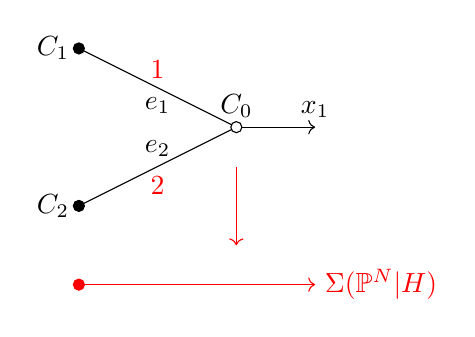
\begin{tikzpicture}
\draw [fill] (0,3) circle[radius=2pt];
\draw (0,3) node[left]{$\mathsq{C}_1$};
\draw (0,3) -- (2,2);
\draw (1,2.5) node[above,color=red]{$1$};
\draw (1,2.5) node[below]{$e_1$};

\draw [fill] (0,1) circle[radius=2pt];
\draw (0,1) node[left]{$\mathsq{C}_2$};
\draw (0,1) -- (2,2);
\draw (1,1.5) node[below,color=red]{$2$};
\draw (1,1.5) node[above]{$e_2$};

\draw [->] (2,2) -- (3,2);
\draw (3,2) node[above]{$x_1$};

\draw [fill=white] (2,2) circle[radius=2pt];
\draw (2,2) node[above]{$\mathsq{C}_0$};

\draw [->,color=red] (2,1.5) -- (2,0.5);

\draw [->,color=red] (0,0) -- (3,0);
\draw (0,0) [fill=red,color=red] circle[radius=2pt];
\draw (3,0) node[right,color=red]{$\Sigma(\PP^N|H)$};
\end{tikzpicture}
\end{center}
Here each edge (corresponding to a node of the curve) has a length $e_i$ and an expansion factor $u_i$ (indicated in red). The moduli space of such tropical maps is generated by the edge lengths $e_1$ and $e_2$
\begin{equation*} (\RR_{\geq 0})_{e_1} \times (\RR_{\geq 0})_{e_2} \end{equation*}
subject to the continuity condition $e_1=2e_2$. So the tropical moduli space is simply $\RR_{\geq 0}$ generated by $e_2$. Note that for any $e_2 > 0$ we have:
\begin{equation*} \lambda(\mathsq{C}_2) = e_2 = e_1/2 < e_1 = \lambda(\mathsq{C}_1). \end{equation*}
Thus, any logarithmic map with combinatorial type given by the above picture is automatically aligned. This means that the map $\VZ \to \Mcal$ is an isomorphism in a neighbourhood of our chosen element (there is no blowing up necessary). Indeed, the tropical moduli space is $\RR_{\geq 0}$ and this cone does not admit a polyhedral decomposition (there is no non-trivial toric blow-up of $\Aaff^1$).
\end{example}

\begin{example}
Consider now an element of $\Mcal$ whose associated tropical map has the corresponding combinatorial type:


\end{example}

\newpage

\section{Recursion formula for $(\PP^N|H)$}

In the previous section we used tropical geometry to identify the logarithmic strata of $\VZ_{1,\alpha}(\PP^N|H,d)$. We now focus our attention on the logarithmic divisors, providing a recursive description for these loci: i.e. a description using a fibre product of smaller moduli spaces. This is the technically most difficult part of the paper. As a result, we obtain a Gathmann recursion formula in genus one.

Note that $f$ has contact order with $H$ exactly equal to $\alpha_k$ at the marking $p_k$, or else the irreducible component of $C$ on which $p_k$ lies is mapped entirely inside $H$. By pulling back along $f$ the equation defining $H$, and taking its $\alpha_k$-th derivative at $p_k$ (which makes sense because all the lower order derivatives do vanish by assumption) we single out the latter locus. By staring at the exact sequence of jet bundles
\[0\to p_k^*\Omega_{C}^{\otimes\alpha_k}\otimes\ev_k^*\OO_{\PP^N}(H)\to p_k^*\mathcal J^{\alpha_k}(f^*\OO_{\PP^N}(H))\to p_k^*\mathcal J^{\alpha_k-1}(f^*\OO_{\PP^N}(H))\to 0\]
we realise that there is on $\VZ_{1,\alpha}(\PP^N|H,d)$ a line bundle (the leftmost term in the exact sequence above) with a natural section cutting the locus where the curve breaks, and the piece containing $p_k$ is mapped inside $H$.
\begin{lem}
 \[(\alpha_k\psi_k+\ev_k^*H)[\VZ_{1,\alpha}(\PP^N|H,d)]=[D_{1,\alpha;k}(\PP^N|H,d)],\]
\end{lem}
In what follows we shall give an explicit (recursive) description of the right-hand side, in terms of tautological classes on spaces of maps with lower numerical invariants.
\begin{remark}
 The divisors we are after are a union of logarithmic strata, because the locus where the log structure is trivial coincides precisely with the nice locus.
\end{remark}
By Corollary \ref{cor:log_smooth}, the logarithmic strata of codimension one correspond to rays of the Artin fan.

\subsection{Combinatorial description}
As long as the minimal subcurve of genus one has positive degree, the picture is classical: the dual graph of the curve is bipartite - vertices mapped inside $H$ are distinguished from the others. In fact there is only one such vertex, because, if there were more, the relative position of their image in $\mathbb R_{\geq 0}$ under the tropical map would be unconstrained, therefore spanning a locus larger than a ray in the tropical moduli space. \marginpar{say something about rigid tropical curves as in ACGS and KLR} We follow in R. Vakil's footsteps in setting the following notation:
\begin{figure}[h]
    \centering
    \begin{minipage}{0.3\textwidth}
        \centering
        \Yagraph
        \caption{$\mathcal Y_a$}
    \end{minipage}\hfill
    \begin{minipage}{0.3\textwidth}
        \centering
        \Ybgraph
        \caption{$\mathcal Y_b$}
    \end{minipage}\hfill
    \begin{minipage}{0.3\textwidth}
        \centering
        \Ycgraph
        \caption{$\mathcal Y_c^+$}
    \end{minipage}
\end{figure}

Notice that continuity of the tropical map determines the mutual relationship among the edge lengths.

On the other hand, when there is a contracted elliptic subcurve - and it will be contracted into the hyperplane, because otherwise it wouldn't be generic, by density of the nice locus in $\VZ_{1,\alpha^\prime}(\PP^N|H,d^\prime)$ - the picture becomes more complicated due to the alignment. The combs may break (multiple times) and they may point in opposite directions. We label these loci $\mathcal{Y}_c^0$.
\begin{figure}
 \tikz{
 \draw (0,0) circle(2pt)[fill=black] (0,2) circle(2pt)[fill=black] (0,4) circle(2pt)[fill=black] (0,6) circle(2pt)[fill=black] (0,-2) circle(2pt)[fill=black] (1.1,1.78) circle(2pt)[fill=black] (3.42,1.42) circle(2pt)[fill=black] (.58,-1.42) circle(2pt)[fill=black];
 \draw (2,0) -- node[above]{4} (0,0) (2,0) --node[above]{2} (1.1,1.78) --node[above]{2} (0,2) (1.1,1.78) --node[above]{1} (0,4) (2,0) --node[above]{1} (3.42,1.42) (2,0) --node[above]{1} (.58,-1.42) (3.42,1.42) --node[above]{5} (0,6) (.58,-1.42) --node[above]{3} (0,-2);
 \draw[red] (2,0) circle(2);
 \draw (2,0) circle(2pt)[fill=white];
 \draw[->] (0,-3) circle(2pt)[fill=black] edge (4,-3);
 }
\end{figure}
\begin{dfn}
 A degree-aligned genus one tropical map $\phi$ to $\mathbb R_{\geq 0}$ is ... with a circle of radius $\delta$ around the core satisfying:
 \begin{enumerate}
  \item the circle of radius $\delta$ passes through at least one vertex of positive degree, and no vertex of positive degree is contained in its strict interior;
  \item every circle of radius $<\delta$ around the core passes through (either none or) at least two vertices;\footnote{The subdivisions we perform before picking a ray correspond to aligning the log structure, i.e. imposing $\lambda(v)=\lambda(v^\prime)$ for some $v,v^\prime$.}
  \item every edge heading out of the circle of radius $\delta$ goes directly to a vertex in $\phi^{-1}(0)$.
 \end{enumerate}
\end{dfn}

\begin{remark}
 The core being contracted in the fiber of the tropical map is not a phenomenon that we should worry about in codimension one. Indeed, assume that the core is contracted in the fiber along a ray. Then all the edges departing from the core have expansion factor $0$; call the corresponding coordinates $U=\{u_i\}_{i\in I}$. Call the remaining coordinates $E=\{e_j\}_{j\in J}$. Note that tropical continuity involves only $E$. Alignments on the other hand assume the form $\lambda(v)=\lambda(v^\prime)$, where $\lambda(v)=\sum_{i\in I(v)}u_i\sum_{j\in J(v)}e_j$. Pick the shortest elements of $U$; then these can be shortened to zero without affecting the rest (by hypothesis, alignments can only identify them among themselves). This shows that we could not have started with a ray.
\end{remark}

\subsection{Explicit realisation}
The description of the first three types is relatively easy:
\begin{enumerate}[label=(\alph*)]
 \item \[\mathcal Y_a=\M{0}{\{-m^{(1)},\ldots,-m^{(r)}\}\cup\alpha^{(0)}}{H}{d_0}^\sim\times_{H^r}\left(\VZc{1}{\alpha^{(1)}\cup\{m^{(1)}\}}{\PP^N|H}{d_1}\times\prod_{i=2}^r\M{0}{\alpha^{(i)}\cup\{m^{(i)}\}}{\PP^N|H}{d_i}\right)\]
 \item \[\mathcal Y_b=\M{0}{\{-m^{(1)},\ldots,-m^{(r)}\}\cup\alpha^{(0)}}{H}{d_0}^\sim\times_{H^r}\left(\M{0}{\alpha^{(1)}\cup\{m^{(1)},m^{(2)}\}}{\PP^N|H}{d_1}\times\prod_{i=3}^r\M{0}{\alpha^{(i)}\cup\{m^{(i)}\}}{\PP^N|H}{d_i}\right)\]
 \item \[\mathcal Y_c^+= \VZc{1}{\{-m^{(1)},\ldots,-m^{(r)}\}\cup\alpha^{(0)}}{H}{d_0}^{\sim} \times_{H^r}\prod_{i=1}^r\M{0}{\alpha^{(i)}\cup\{m^{(i)}\}}{\PP^N|H}{d_i}\]
\end{enumerate}
where $\M{0}{\mu}{H}{d}^\sim$ denotes the space of genus zero punctured maps, while $\VZc{0}{\mu}{H}{d}$ denotes the desingularisation of the main component of the space of punctured maps discussed in Section ???. The numerical data run over all splitting $A$ of the tangency conditions (resp. $B$ of the degree) in $r+1$ parts, such that:
\begin{enumerate}
 \item $d_0+\sum_{i=1}^r m^{(i)}=\sum\alpha^{(0)}$;
 \item $d_i=m^{(i)}+\sum\alpha^{(i)}$;
 \item $d_0>0$ in case $c$.
\end{enumerate}

Review here the process of gluing for punctured maps. In particular the basic monoid should be modified in order to make the relevant evaluations log morphisms. Claim: evaluations are strict. Consequence: the fiber product in the category of log stacks is fine. We have then to apply saturation. This is a finite morphism of degree... (I think it could be $\frac{\prod m^{(i)}}{lcm(m^{(i)})}$).

\begin{lemma}[Virtual pushforward] The following hold.
 \begin{itemize}
  \item $\fgt_*[\M{0}{\alpha}{\PP^N|H}{d}]=[\MG{0}{\alpha}{\PP^N|H}{d}]$ (follows from \cite{GathmannThesis,AbramovichMarcusWiseComparison}).
  \item $\fgt_*[\VZc{1}{\alpha}{\PP^N|H}{d}]$ computes the reduced relative invariants by definition.
  \item $\fgt_*[\M{0}{\mu}{H}{d_0}^\sim]=[\M{0}{\lvert\mu\rvert}{H}{d_0}]$ (follows from \cite{GathmannThesis} and... comparison of punctured with rubber invariants).
  \item $\fgt_*[\VZc{1}{\mu}{H}{d_0}^\sim]$ here we should need a variation on Pixton's DRC formula; hopefully it's enough to avoid the graphs that tropical well-spacedness discards.
 \end{itemize}
\end{lemma}

\subsection{$\mathcal{Y}_c^0$}
\begin{ex}
 We look at the following example in some detail.
 \begin{figure}[h]
  \tikz{
  \draw (0,1) circle(2pt)[fill=black] --node[above]{2} (2,0);
  \draw (0,-1) circle(2pt)[fill=black] --node[above]{2} (2,0);
  \draw (2,0) -- (2.5,0) node[right]{4};
  \draw (2,0)  circle(2pt)[fill=white];
  \draw (0,1) -- (.33,1.33) node[above right]{0};
  \draw (0,-1) -- (.33,-1.33) node[below right]{0};
  \draw[red] (2,0) circle(2.23);
  \draw[->] (0,-2.5)node[left]{0} circle(2pt)[fill=black] edge (4,-2.5);
  }
 \end{figure}
 The ambient space is $\VZc{1}{(4,0,0)}{\PP^N|H}{4}$, of dimension $4N+3$. The underlying moduli space is $X=\M{0}{(2,0)}{\PP^N|H}{2}\times_H\M{0}{(2,0)}{\PP^N|H}{2}\times\VZ_{1,(-2,-2,4)}$ of dimension $5N+1$. Consider the fiber product:
 \bcd
 F\ar[r]\ar[d]& \M{0}{(2,0)}{\PP^N|H}{2}\times\M{0}{(2,0)}{\PP^N|H}{2}\ar[d]\\
 H\ar[r] & H\times H
 \ecd
 At the level of ghost sheaves, $\oM_F=\mathbb N\oplus_{\mathbb N^2}\oM_1^{\rm{enl}}\oplus\oM_2^{\rm{enl}}$, where the map $\mathbb N^2\to\mathbb N$ is the sum, and the map $\mathbb N^2\to\oM_1^{\rm{enl}}\oplus\oM_2^{\rm{enl}}$ generically is multiplication by $2$, so $\oM_F=\mathbb N^2/(2e=2f)$ generically. Saturation gives a finite cover $G\to F$ with $\oM_G=\mathbb N_{e=f}$ generically. Lifting this to actual log structures, what we are doing (again generically) is taking a square root of the isomorphism $T_{R_1,q_1}^{\otimes 2}\simeq T_{R_2,q_2}^{\otimes 2}$, which is obtained passing through $N_{H/\PP^N,f(Z)}$ via $\operatorname{d}f_{|R_i,q_i}$. This breaks when $f_{|R_i}$ is not tangent to $H$ of order exactly $2$ at $q_i$, for either $i$; but by the maximality assumption this happens precisely along Gathmann's comb loci $\Delta_i$. So in fact, rather than with $T_{R_i,q_i}^{\otimes 2}$, we should be working with $T_{R_i,q_i}^{\otimes 2}(-\Delta_i)$: but this is exactly $\ev_i^*(-H)$ by Gathmann's genus zero formula, and the isomorphism $\ev_1^*(H)=\ev_2^*(H)$ holds on all of $F$.
 
 On the other hand, generically on $\VZ_{1,(-2,-2,4)}$ we have $T_{q_1}Z\simeq T_{q_2}Z$ by exploiting the group structure on the elliptic curve. This breaks when either (but not both) is on a rational tail. Yet we have $T_{q_1}Z(\Delta_{1\in P})\simeq T_{q_2}Z(\Delta_{2\in P})$ by Vakil-Zinger's construction of a universal $\psi$-class (i.e. by comparing both with $\pi_*\omega(\Delta)$; notice that our further blow-up has the only effect of twisting \emph{all} the relevant line bundles by $\Delta_{1,2\notin P}$).
 
 Now, the fiber of the Vakil-Zinger blow-up over $X$ can be described as follows. Generically it looks like \[\PP(T_{q_1}R_1\otimes T_{q_1}Z\oplus T_{q_2}R_2\otimes T_{q_2}Z)\]
 but this has to be modified along the boundary:
 \begin{itemize}
  \item this has to do with the fact that the normal bundle of the strict transform is the pullback of the normal bundle twisted by the intersection with the exceptional divisor (so it relates with previous steps of the blow-up);
  \item it is not globally a $\PP^1$-bundle (so it relates with further stages of the blow-up; it also has to do with a choice of compactification for the moduli space of attachments);
  \item it has the effect of replacing $T_{q_i}Z$ with Vakil-Zinger's universal $\mathbb T$, so that this can be factored out of the projective bundle, and in fact we are left with a projective bundle $\mathbb P=\PP(T_{q_1}R_1\oplus T_{q_2}R_2)$ over $F$, and its open part $\operatorname{Iso}(T_{q_1}R_1\oplus T_{q_2}R_2)$ represents the attachment data for a contraction to a tacnode $R_1\sqcup_q R_2\to\bar{C}$.
 \end{itemize}
On $\PP$ there is a natural vector bundle map \[s\colon \OO_{\PP}(-1)\hookrightarrow p^*(T_{q_1}R_1\oplus T_{q_2}R_2)\xrightarrow{+\operatorname{d}f}\ev_q^*T\PP^N\]
that vanishes along the locus where $f$ descends to $\bar C$. In general, it is not a transversal section:
\begin{itemize}
 \item we should replace $T\PP^N$ by $TH$ as long as all the $m^{(i)}$ are $\geq2$;
 \item Vakil and Zinger construct a blow-up of $\PP$ along the vanishing loci of $s$ of low codimension, and twist $s$ by the exceptional divisors, so that it becomes a transverse section $\tilde{s}$.
\end{itemize}
On the other hand, the finite cover $G\to F$ factors through $\PP$, because the two vertices are already aligned on $G$. We claim that the boundary locus of $\VZc{1}{(4,0,0)}{\PP^N|H}{4}$ corresponding to the combinatorial type of the tropical map above is the transverse intersection
\[\left(G\cap V(\tilde{s})\subseteq\PP\right)\times\VZ_{1,(-2,-2,4)}.\]
This has the expected dimension (codimension $N-1$ with respect to $X$). To compute its class, we can pull $\PP$ back to $G$, and then notice that $G\hookrightarrow\PP_G$ is the inclusion of a (trivial) subbundle.
\begin{lem}
 The class of $\PP(\mathcal F)\subseteq\PP(\mathcal E)$ is $c_{\rm{top}}(\OO_\mathcal{E}(1)\otimes p^*(\mathcal{E}/\mathcal{F}))$.
\end{lem}
See \cite[Prop. 9.13]{EH3264}. It is a good time to remember that $\mathcal E$ was in fact $(\bigoplus_{i=1}^rTR_{i,q_i})\otimes\mathbb T$. By writing $c$ for $c_1(\OO_\mathcal{E}(1))$, $\psi_i$ for $c_1(T^*R_{i,q_i})$, $\psi_Z$ for Vakil-Zinger's universal psi class, and $H$ for $\ev_q^*H$, we need to compute
\begin{align*}
p_*\left((c-\psi_1-\psi_2-2\psi_Z)[(1+c+H)^N(1+c)^{-1}]_{N-1}\right)= \\
p_*\left((c-\psi_1-\psi_2-2\psi_Z)(\sum_{k=0}^{N-1}\binom{N}{1+k}c^kH^{N-1-k})\right)=\\
\sum_{k=0}^{N-1}\binom{N}{k}H^{N-1-k}\big(s_k(\mathcal E)-s_{k-1}(\mathcal E)(\psi_1+\psi_2+\psi_Z)\big)
\end{align*}
\end{ex}

\section{Recursion formula in general}
Now let $(X|Y)$ be a smooth pair with $Y$ very ample. The complete linear system $|\OO_X(Y)|$ defines an embedding $X \hookrightarrow \PP^N$ with $Y=X\cap H$ for $H$ some hyperplane.

\begin{lemma} The following square is cartesian (in the category of ordinary stacks):
\bcd
\VZ_{1,\alpha}(X|Y,\beta) \ar[r] \ar[d] \ar[rd,phantom,"\square"] & \VZ_{1,\alpha}(\PP^N|H,d) \ar[d] \\
\VZ_{1,n}(X,\beta) \ar[r,"i"] & \VZ_{1,n}(\PP^N,d).
\ecd
\end{lemma}
Since $\VZ_{1,n}(\PP^N,d)$ is smooth and $\VZ_{1,n}(X,\beta)$ carries a natural virtual class, there is a diagonal pull-back morphism which we use to define the virtual class on the space of maps to $(X|Y)$:
\begin{equation*} \virt{\VZ_{1,\alpha}(X|Y,\beta)} := i_\Delta^! [\VZ_{1,\alpha}(\PP^N|H,d)]. \end{equation*}
The recursion formula in $\VZ_{1,\alpha}(\PP^N|H,d)$ immediately pulls back along $i$ to give a recursion formula in $\VZ_{1,\alpha}(X|Y,\beta)$. \footnote{(Navid) Is it clear how to compute integrals over the pulled back classes?}


\section{Quantum Lefschetz in genus one}



\bibliographystyle{alpha}
\bibliography{Bibliography}

\bigskip\bigskip

\noindent Luca Battistella\\
Department of Mathematics, Imperial College London \\
\texttt{l.battistella14@imperial.ac.uk}\\

\noindent Navid Nabijou \\
Department of Mathematics, Imperial College London \\
\texttt{navid.nabijou09@imperial.ac.uk}\\

\noindent Dhruv Ranganathan \\
Department of Mathematics, Massachusetts Institute of Technology \\
\texttt{dhruvr@mit.edu}


\end{document}